\chapter{METODOLOGIA}
Neste trabalho, a abordagem metodológica para o estudo do controle de trajetória em impressoras 3D, aplicando algoritmos iterativos e técnicas de programação não linear, é estruturada em duas etapas fundamentais. A primeira etapa envolve a elaboração de um modelo computacional que representa o comportamento mecânico da impressora 3D, integrando o método avançado de controle de trajetória baseado em programação não linear proposto neste estudo. A última fase é dedicada à realização de simulações computacionais, as quais são utilizadas para avaliar o desempenho do método de controle.

O processo metodológico é visualizado de forma esquemática no fluxograma abaixo (Figura \ref{fig:fluxo_geral}), o qual esclarece as etapas consecutivas desde a geração do comando até a geração dos sinais de controle, enfatizando a aplicação do modelo desenvolvido na fase de controle de trajetória.

\begin{figure}[H]
    \centering
    \caption{Fluxograma geral das etapas para o controle de trajetória}
    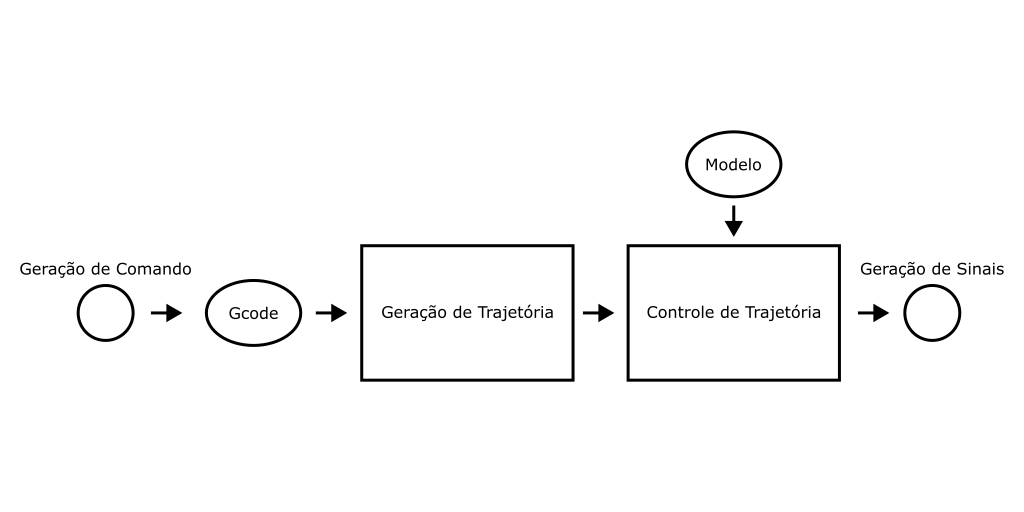
\includegraphics[scale=0.4]{fluxo_geral}

    \label{fig:fluxo_geral}
\end{figure}

\section{Geração de Trajetória}

A fase de geração de trajetória inicia-se com a análise do Gcode, que fornece as coordenadas e velocidades de destino dos movimentos. Neste processo, são considerados exclusivamente os comandos G1, que indicam movimentos lineares, e são extraídas as informações referentes aos eixos X, Y e à taxa de avanço (\textit{feedrate} - F). É importante notar que a taxa de avanço, usualmente expressa em milímetros por minuto nos arquivos Gcode gerados por fatiadores, é convertida para milímetros por segundo.

\begin{figure}[H]
    \centering
    \caption{Curva de velocidade trapezoidal}
    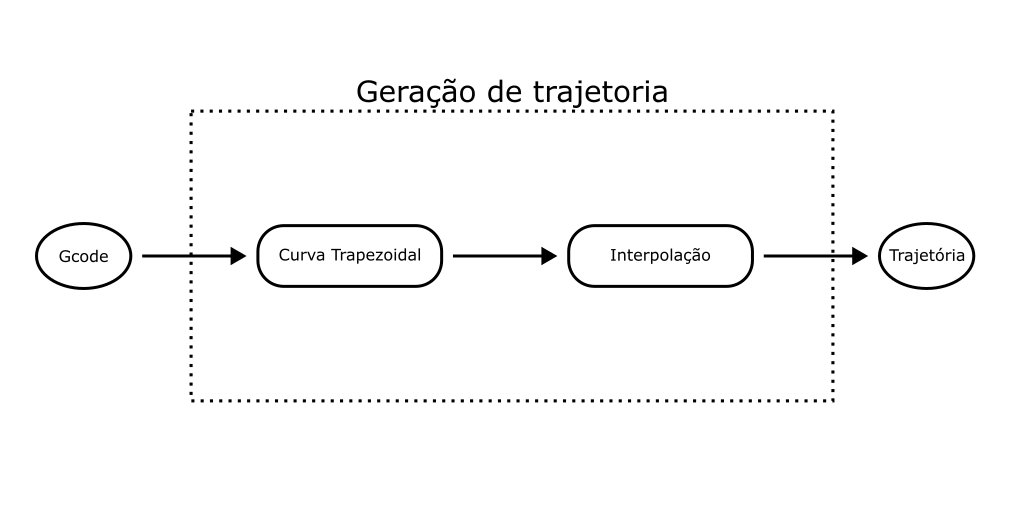
\includegraphics[scale=0.4]{geracao_de_trajetoria}

    \label{fig:geracao_de_trajetoria}
\end{figure}

\subsection{Curva trapezoidal de velocidade}

A próxima etapa  envolve a elaboração da curva trapezoidal de velocidade. Esta etapa se baseia em dados de entrada como deslocamento, velocidades iniciais e finais, e a velocidade almejada. A execução desta velocidade desejada é avaliada através do cálculo da velocidade de pico \(v_p\). Tal velocidade é obtida pela interseção das trajetórias de aceleração e desaceleração, que iniciam nas velocidades iniciais e finais respectivamente, e considerando que a área sob a curva deve ser equivalente ao deslocamento requerido. A fórmula para calcular \(v_p\) é expressa pela Equação \ref{eq:v_p}:

\begin{equation}
    \label{eq:v_p}
    v_p = \sqrt{\frac{(v_1^2+v_2^2)}{2}+a d}
\end{equation}

Nesta equação, \(v_1\) e \(v_2\) representam as velocidades iniciais e finais, \(a\) denota a aceleração definida na impressora, e \(d\) corresponde ao deslocamento.

A comparação entre a velocidade de pico e a velocidade desejada, esta última estabelecida pelo \textit{feedrate} no Gcode, é crucial para definir se a trajetória do movimento adotará um perfil trapezoidal ou triangular de velocidade. A configuração do perfil depende da relação entre a velocidade de pico e a velocidade desejada: caso a primeira seja superior, o movimento será estruturado em três segmentos distintos, conforme ilustrado na Figura \ref{fig:trap_curv}.

\begin{figure}[H]
    \centering
    \caption{Curva de velocidade trapezoidal}
    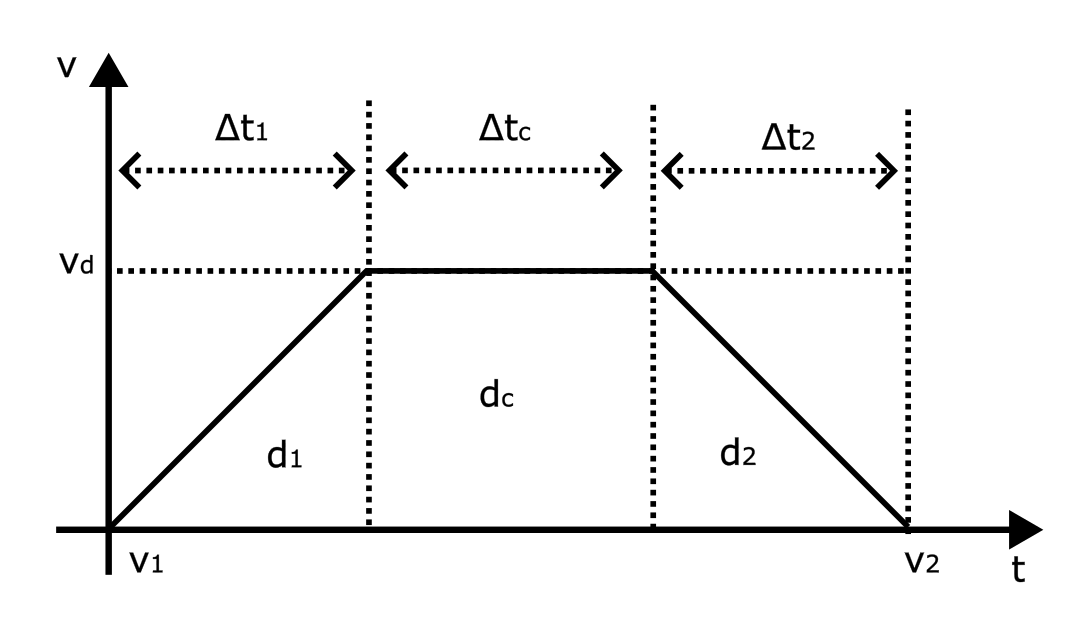
\includegraphics[scale=0.4]{trap_curv}
    \label{fig:trap_curv}
\end{figure}

Os segmentos de deslocamento \(d_1\), \(d_2\), e \(d_c\) correspondem às fases de aceleração, velocidade constante e desaceleração do movimento, respectivamente, e devem totalizar \(d\), o deslocamento total necessário. As variações temporais \(\Delta t_1\), \(\Delta t_2\), e \(\Delta t_c\) representam as durações de cada fase, baseadas nas velocidades inicial (\(v_1\)) e final (\(v_2\)), e na velocidade desejada (\(v_d\)). Os deslocamentos parciais são determinados pelas equações abaixo (Equação \ref{eq:des_seg_1_trap},  \ref{eq:des_seg_2_trap} e  \ref{eq:des_seg_c_trap}), que levam em conta a aceleração \(a\):

\begin{equation}
    \label{eq:des_seg_1_trap}
    d_1 = \frac{(v_d^2-v_1^2)}{(2 a)}
\end{equation}

\begin{equation}
    \label{eq:des_seg_2_trap}
    d_2 = \frac{(v_2^2-v_d^2)}{(2 a)}
\end{equation}

\begin{equation}
    \label{eq:des_seg_c_trap}
    d_c = d-(d_1+d_2)
\end{equation}

Os intervalos de tempo para as fases de aceleração, velocidade constante e desaceleração são calculados conforme (Equação \ref{eq:dt_seg_1_trap},  \ref{eq:dt_seg_2_trap} e  \ref{eq:dt_seg_c_trap}):

\begin{equation}
    \label{eq:dt_seg_1_trap}
    \Delta t_1 = \frac{(v_d-v_1)}{a}
\end{equation}

\begin{equation}
    \label{eq:dt_seg_2_trap}
    \Delta t_2 = \frac{(v_2-v_d)}{a}
\end{equation}

\begin{equation}
    \label{eq:dt_seg_c_trap}
    \Delta t_c = \frac{d_c}{v_d}
\end{equation}

Quando a velocidade de pico (\(v_p\)) é inferior à velocidade desejada (\(v_d\)), o perfil da trajetória de movimento assume uma forma triangular, em vez de trapezoidal. Esta condição implica que a velocidade desejada não é atingida durante o comando e, por conseguinte, o movimento é caracterizado por uma aceleração constante seguida de uma desaceleração constante, sem fase de velocidade constante. A Figura \ref{fig:triang_curv} ilustra este perfil de velocidade triangular.

\begin{figure}[H]
    \centering
    \caption{Curva de velocidade triangular}
    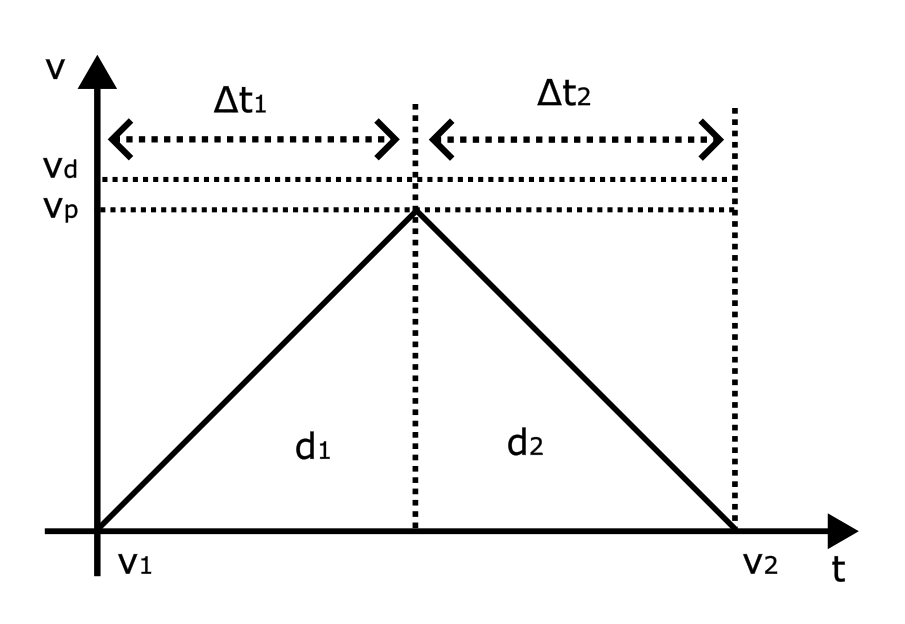
\includegraphics[scale=0.4]{triang_curv}

    \label{fig:triang_curv}
\end{figure}

Neste cenário, os segmentos de deslocamento \(d_1\) e \(d_2\) representam, respectivamente, as etapas de aceleração até a velocidade de pico e a desaceleração de volta à velocidade final. Os valores de \(d_1\) e \(d_2\) são calculados pelas seguintes equações (Equação \ref{eq:des_seg_1_tri}, \ref{eq:des_seg_2_tri}), que incorporam a aceleração (\(a\)) e as velocidades inicial (\(v_1\)) e final (\(v_2\)):

\begin{equation}
    \label{eq:des_seg_1_tri}
    d_1 = \frac{(v_p^2-v_1^2)}{(2 a)}
\end{equation}

\begin{equation}
    \label{eq:des_seg_2_tri}
    d_2 = \frac{(v_2^2-v_p^2)}{(2 a)}
\end{equation}

É possível calcular os intervalos de tempo dessas fases, através das Equações \ref{eq:dt_seg_1_tri} e \ref{eq:dt_seg_2_tri}.

\begin{equation}
    \label{eq:dt_seg_1_tri}
    t_1 = \frac{(v_p-v_1)}{a}
\end{equation}

\begin{equation}
    \label{eq:dt_seg_2_tri}
    t_2 = \frac{(v_2-v_p)}{a}
\end{equation}

Onde os tempos \(t_1\) e \(t_2\) representam, respectivamente, o tempo necessário para acelerar de \(v_1\) a \(v_p\) e para desacelerar de \(v_p\) a \(v_2\). 

Esses passos transformam a sequência de comandos movimentos do Gcode em uma trajetória com pontos com informações do deslocamento, velocidade, tempo, definidos nos nós onde ha alteração na aceleração, estabelecendo o comportamento dos movimentos de x e y no tempo.

\subsection{Interpolação}
A interpolação é um passo crucial para refinar a trajetória de movimento na impressão 3D. Esta fase trabalha sobre a trajetória definida para cada eixo na etapa anterior, empregando uma função de interpolação que gera pontos intermediários. Esses pontos são criados com base em um intervalo de tempo previamente definido, melhorando significativamente a resolução da trajetória.

Para subdividir esses intervalos de maneira eficaz, a Equação \ref{eq:N_steps} é utilizada para calcular o número de passos de interpolação necessários:

\begin{equation}
    \label{eq:N_steps}
    N = \lceil\frac{\Delta t}{\Delta p}-1\rceil
\end{equation}

Esta fórmula determina o número \( N \) de passos a serem tomados dentro de um dado intervalo de tempo \( \Delta t \), com cada passo tendo um período \( \Delta p \). Após a divisão dos intervalos, a Equação \ref{eq:dt_interpol_last_step} calcula o tempo restante no último passo de interpolação (\(\Delta t_f\)):

\begin{equation}
    \label{eq:dt_interpol_last_step}
    \Delta t_f= \Delta t - \Delta p N 
\end{equation}

Finalmente, com base nesses passos de tempo determinados (\(\Delta t_i\)) anexando \(\Delta t_f\) à lista de passos \(\Delta p\) de tamanho \(N\), a Equação \ref{eq:delta_des_interpol} é empregada para calcular o deslocamento correspondente a cada passo (\(\Delta d_i\)), utilizando a aceleração do segmento a ser interpolado (\(a_s\)) e a velocidade inicial do segmento (\(v_s\)):

\begin{equation}
    \label{eq:delta_des_interpol}
    \Delta d_i = \Delta v_s \Delta t_i+ \frac{a_s \Delta t_i^2}{2} 
\end{equation}

Esses cálculos são fundamentais para garantir que a trajetória seja suficientemente detalhada, permitindo que a fase de controle da trajetória seja executada com sucesso.

\section{Modelagem dinâmica de uma impressora 3D} 
\label{sec:modelagem}

A modelagem do sistema mecânico da impressora 3D é um passo crucial para a implementação eficaz do método proposto. Essa modelagem não só facilita a compreensão do comportamento da impressora mas também é fundamental para definir as restrições necessárias na etapa subsequente de controle de trajetória, restrições essas que aplicam as equações de movimento e condições de contorno definidas no modelo.

É fundamental enfatizar a importância de um modelo representativo. A eficácia do método proposto depende diretamente da acurácia com que o modelo simula o comportamento real da impressora 3D. Neste estudo, consideramos as seguintes características principais do sistema (Figura \ref{fig:simple_model}):

\begin{itemize}
    \item Influência da Correia: A correia é o componente chave responsável por introduzir desvios nas trajetórias de impressão. Ela age como uma combinação de mola e amortecedor, afetando a dinâmica do movimento.
    \item Modelagem do Conjunto Bico Injetor e Extrusora: Este conjunto é tratado como um corpo rígido uniforme, simplificando sua representação geométrica.
    \item Dimensões da Mesa de Impressão: A área útil da mesa de impressão é de 200 mm x 200 mm, definindo o espaço de trabalho disponível.
    \item Configuração Cartesiana: A impressora opera em um sistema cartesiano, com eixos ortogonais, o que simplifica a análise de movimento.
    \item Independência dos Eixos: Cada eixo da impressora opera independentemente dos outros, permitindo uma análise mais simplificada das dinâmicas individuais.
    \item Condições Iniciais de Movimento: Assume-se que todos os movimentos da impressora iniciam a partir do estado de repouso.
\end{itemize}

\begin{figure}[H]
    \centering
    \caption{Modelo simplificado impressora 3D}
    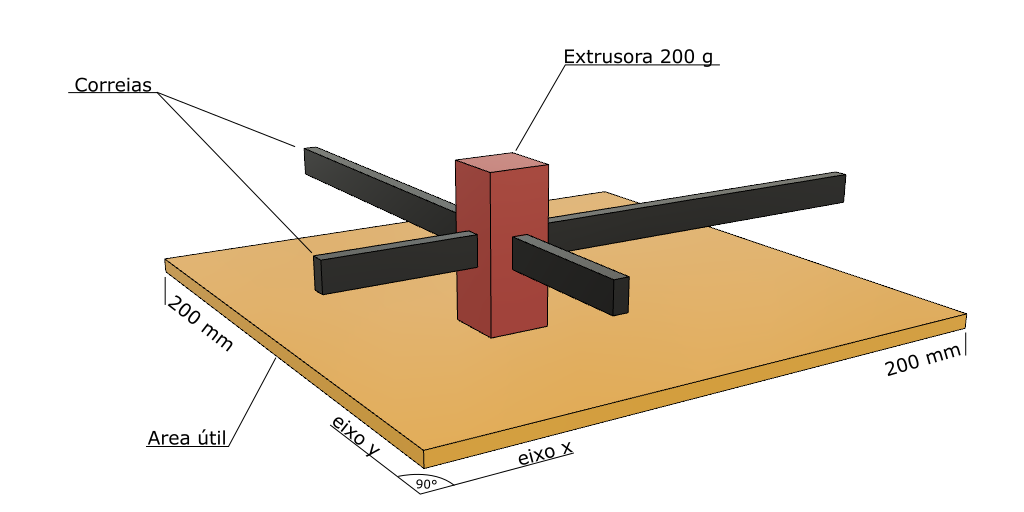
\includegraphics[scale=0.58]{simple_model}
    \label{fig:simple_model}
\end{figure}

Com base nesses parâmetros, definimos duas posições-chave para análise em cada eixo. A primeira é a posição ideal (\(x_b\)) ou posição da base, que representa o ponto desejado pelo usuário, assumindo um sistema sem flexibilidade ou perdas. A segunda é a posição real (\(x_p\)) ou a posição da ponta, que leva em conta as forças inerciais e a flexibilidade introduzida pela correia. Este modelo é ilustrado na figura \ref{fig:model_1_axis}.

\begin{figure}[H]
    \centering
    \caption{Modelagem de 1 eixo}
    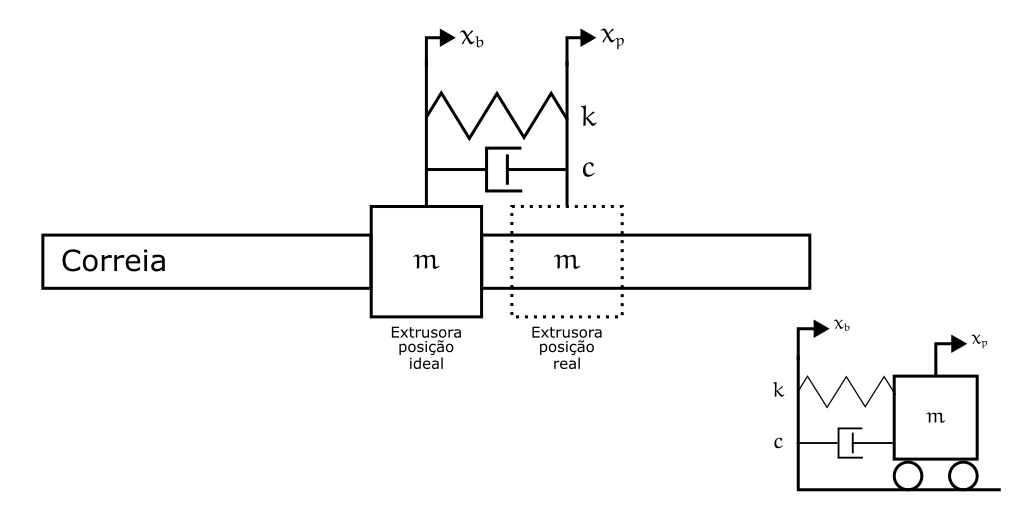
\includegraphics[scale=0.4]{model_1_axis}

    \label{fig:model_1_axis}
\end{figure}

As equações de movimento para a impressora são descritas a seguir (Equações \ref{eq:mov_impressora_1} e \ref{eq:mov_impressora_2}):

\begin{equation}
    \label{eq:mov_impressora_1}
    m \ddot{x_p} + c(\dot{x_p} - \dot{x_b}) + k(x_p-x_b) = 0 
\end{equation}

\begin{equation}
    \label{eq:mov_impressora_2}
    \ddot{x_p} = \frac{c}{m}(\dot{x_b} - \dot{x_p}) + \frac{k}{m}(x_b - x_p) 
\end{equation}

Nestas equações, \(m\) representa a massa do conjunto bico injetor e extrusora, \(c\) é a constante de amortecimento da correia, e \(k\) é a constante da mola equivalente da correia. As variáveis \(x_p\) e \(x_b\) correspondem, respectivamente, às posições da ponta e da base do componente em movimento. 

Este modelo dinâmico pode ser representado por dois parâmetros, a frequência natural e o coeficiente de amortecimento, que se relacionam através das Equações \ref{eq:freq_nat}.


\begin{equation}
    \label{eq:freq_nat}
    \omega = \sqrt{\frac{k}{m}}
\end{equation}

\begin{equation}
    \label{eq:amort}
    \zeta = \frac{c}{2mk}
\end{equation}

\begin{equation}
    \label{eq:equation_simpl}
    \ddot{x_p} = 2 \zeta \omega(\dot{x_b} - \dot{x_p}) + \omega ^2(x_b - x_p)
\end{equation}

Essas equações fundamentam o modelo dinâmico que empregamos para simular e otimizar a trajetória de impressão na impressora 3D. Na Figura \ref{fig:model_2_axis} é representada a composição dos eixos x e y utilizado neste estudo, sendo considerada a aplicação das Equação \ref{eq:mov_impressora} para cada um dos eixos de maneira análoga, podendo identificar o eixo através dos subíndices \(x\) e \(y\), ou no caso das posições o eixo y é identificado por \(y_p\) e \(y_b\) (posição da ponta do eixo y e posição da base do eixo y respectivamente).

\begin{figure}[H]
    \centering
    \caption{Modelagem dos eixos x e y}
    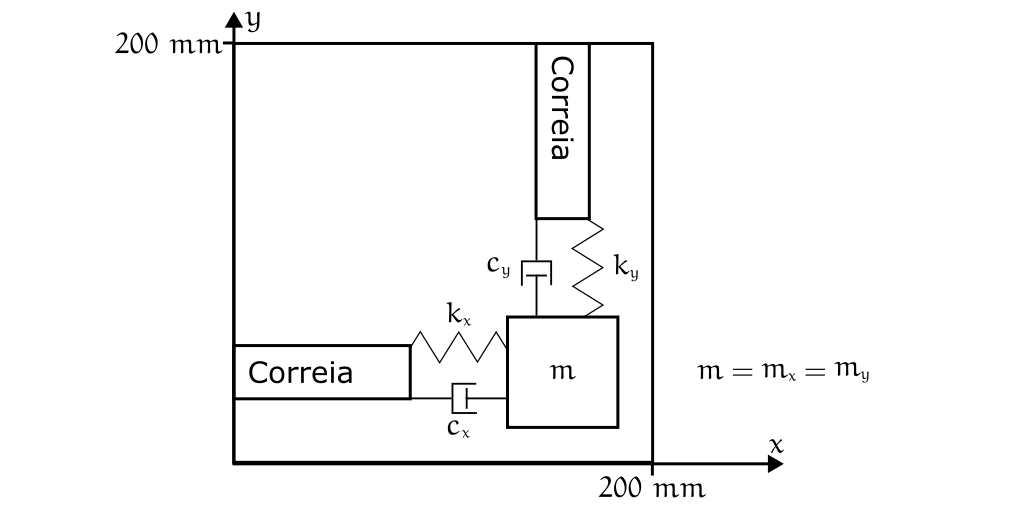
\includegraphics[scale=0.4]{model_2_axis}

    \label{fig:model_2_axis}
\end{figure}

\subsection{Espaço de estados}
A formulação do espaço de estados é adotada neste estudo para simplificar as operações e a solução do sistema dinâmico da impressora 3D. Esta abordagem é eficaz pois transforma uma equação diferencial de ordem superior em um sistema de equações diferenciais de primeira ordem, mas com um número maior de equações. Esta metodologia facilita o entendimento e a manipulação das dinâmicas do sistema.

O modelo dinâmico no espaço de estados é representado na seguinte forma (Equação \ref{eq:simp_state_space_din_model}):

\begin{equation}
    \label{eq:simp_state_space_din_model}
    \dot x = A*x+B*u
\end{equation}

Nesta equação, \(\dot x\) representa o vetor de estados derivados, \(x\) é o vetor de estados, \(A\) é a matriz do sistema que define a relação entre os estados atuais e suas taxas de mudança, \(u\) é o vetor de entradas externas, e \(B\) é a matriz de controle que relaciona as entradas com os estados.

Baseado na equação de movimento \ref{eq:mov_impressora}, análogos ao eixo y, expandimos as matrizes e vetores para representar com precisão a dinâmica do sistema no espaço de estados, conforme apresentado na equação \ref{eq:espaco_de_estados_din_model}:

\begin{equation}
    \label{eq:espaco_de_estados_din_model}
    \begin{bmatrix}
        \dot{x_p} \\
        \dot{y_p} \\
        \ddot{x_p} \\
        \ddot{y_p}
    \end{bmatrix}
    =
    \begin{bmatrix}
        0 & 0 & 1 & 0 \\
        0 & 0 & 0 & 1 \\
        -\omega _x ^2 & 0 & -2 \zeta _x \omega _x & 0 \\
        0 & -\omega _y ^2 & 0 & -2 \zeta _y \omega _y
    \end{bmatrix}
    \begin{bmatrix}
        x_p \\    
        y_p \\
        \dot{x_p} \\    
        \dot{y_p} \\
    \end{bmatrix}
    +
    \begin{bmatrix}
        0 & 0 & 0 & 0 \\
        0 & 0 & 0 & 0 \\
        \omega _x ^2 & 0 & 2 \zeta _x \omega _x & 0 \\
        0 & \omega _y ^2 & 0 & 2 \zeta _y \omega _y
    \end{bmatrix}
    \begin{bmatrix}
        x_b \\
        y_b \\
        \dot{x_b}  \\
        \dot{y_b} 
    \end{bmatrix}
\end{equation}

Nesta equação, \(x_p\) e \(y_p\) são as posições reais (da ponta) nos eixos X e Y, respectivamente, enquanto \(x_b\) e \(y_b\) são as posições ideais (da base). As variáveis \(\dot{x_p}\) e \(\dot{y_p}\) representam a primeira derivada do tempo das posições nos eixos X e Y, indicando a velocidade e aceleração. \(\omega _x\) e \(\omega _y\) denotam as frequências naturais do sistema nos eixos X e Y respectivamente, enquanto \(\zeta _x\) e \(\zeta _y\) representam os coeficientes de amortecimento dos mesmos.

\section{Controle de Trajetória}
O Controle de Trajetória desempenha um papel essencial em aperfeiçoar a precisão dos movimentos na impressora 3D. A escolha das estratégias de controle é crucial para maximizar a eficiência operacional. No escopo deste estudo, a técnica de controle adotada se baseia no modelo estabelecido anteriormente, onde aplicamos uma abordagem \textit{feedforward} à trajetória gerada na fase de construção da trajetória.

A metodologia de controle em foco procura resolver as equações de movimento e atender às condições de contorno estipuladas pela modelagem da impressora. O ajuste é feito na trajetória da base do sistema, ajustando-a de forma que a saída do vetor de estados corresponda à trajetória da ponta projetada.

Utiliza-se uma função de otimização iterativa para refinar a trajetória da base, que é a principal variável de interesse. Este refinamento é feito minimizando um conjunto de restrições derivadas das equações de movimento e das condições de contorno. A iteração prossegue até que um critério de parada estabelecido seja alcançado, sugerindo que a trajetória base modificada satisfaz a trajetória da ponta almejada.

Este método assegura uma resposta proativa às dinâmicas da impressora, alinhando-se à trajetória planejada e, consequentemente, elevando a acuidade dos movimentos da impressora 3D. A Figura \ref{fig:controle_de_trajetoria} ilustra o esquema do método de controle proposto.

\begin{figure}[H]
    \centering
    \caption{Fluxograma Controle de Trajetória}
    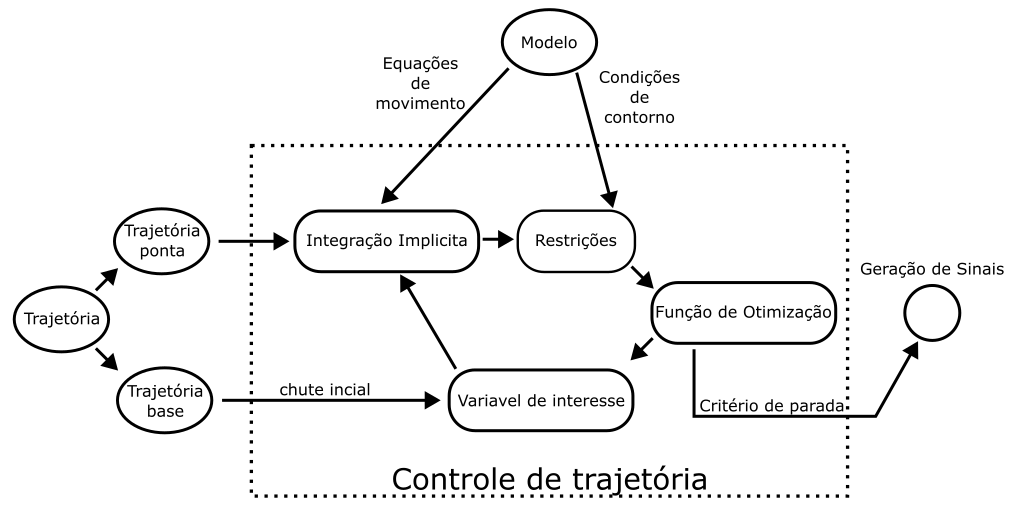
\includegraphics[scale=0.5]{controle_de_trajetoria}

    \label{fig:controle_de_trajetoria}
\end{figure}

\subsection{Restrições}

A formulação do conjunto de restrições é um componente crucial do método, pois é através dele que as equações de movimento são implementadas. A função de otimização adota um algoritmo para minimizar essas restrições, ou seja, para que se aproximem tanto quanto possível de zero.

As condições de contorno são aplicadas estabelecendo que tanto a posição quanto a velocidade sejam zero no instante inicial e que a velocidade também seja zero ao final do percurso. As equações de movimento são incorporadas nas restrições através do método de programação não linear descrito na Seção \ref{sec:hargraves}. Com base no modelo em espaço de estados especificado na Seção \ref{sec:modelagem}. Utilizamos as Equações \ref{eq:state_center_segment}, \ref{eq:state_dot_center_segment}, \ref{eq:input_value_center_segment} e \ref{eq:defect_calc} para criar um vetor de defeitos, como descrito no Capítulo \ref{sec:hargraves}. A minimização destas diferenças faz com que os polinômios cúbicos dos segmentos da curva se aproximem das soluções das equações de movimento, que são então integradas ao vetor de restrições.

\subsection{Função de Otimização}

Os limites da variável de interesse, que neste caso são determinados pela área de trabalho da impressora, também são definidos para que a extrusora não ultrapasse os limites da base de impressão, estabelecendo-se entre o mínimo de 0 e o máximo de 200 mm para os eixos x e y.

A função de otimização adota o algoritmo interior-point, eficaz em resolver problemas de otimização não-linear com restrições. Este método é preferível para grandes conjuntos de dados, por ser mais rápido e numericamente estável do que abordagens tradicionais. Os critérios de parada para o algoritmo são apresentados na Tabela \ref{tab:stop_crit}.

\begin{table}[H]
    \centering
    \caption{Critérios de Parada do Algoritmo de Otimização}
    \label{tab:stop_crit}
    \begin{tabular}{c c}
        Opção & Valor \\ \hline
        Máximo de Iterações & 100000 \\
        Diferença Mínima entre Iterações & 0.0001 \\ \hline
    \end{tabular}
\end{table}
